\documentclass[a4paper,11pt]{article}
\usepackage{CJK} %使用CJK套件
\usepackage{indentfirst} %段首缩进
\usepackage{graphicx}
\usepackage{booktabs}
%\usepackage[T1]{fontenc}
\usepackage{xcolor}
\usepackage{listings}

\author{Dannoy.Lee \\
    dannoy.lee@gmail.com
    }
% define the title
\title{Details of Android Binder IPC System}
\begin{document}
%\begin{CJK}{UTF8}{bsmi} %開始CJK環境,設定編碼,設定字體
%\hbadness=10000

%\tolerance=10000

%\hfuzz=150pt
\begin{CJK*}{UTF8}{gbsn}
%\pagestyle{headings}
%设置listings的全局属性(包含代码)
\lstset{numbers=left, numberstyle=\tiny, keywordstyle=\color{blue!70}, commentstyle=\color{red!50!green!50!blue!50}, frame=shadowbox, rulesepcolor=\color{red!20!green!20!blue!20}}
% generates the title
\maketitle

% insert the table of contents
\tableofcontents
\newpage

\section{引言}
Binder是Android系统进程间通信(IPC)方式之一。深入了解Binder并将之与传统 IPC做对比有助于我们深入领会进程间通信的实现和性能优化。 

本文试图对Android系统的的IPC通信机制的基石--binder进行较详细的分析。但由于对Andrid平台环境不够熟悉以及能力上的限制,理解上可能会出现偏差。
    \subsection{概念}
    \begin{enumerate}
        \item IPC \\
        IPC(Inter-Process Communication,进程间通信),顾名思意是在同一台机器之上不同进程之间通信的方法。
        在linux平台上现有的方式有:信号,管道(命名与匿名),信号量,共享内存,消息队列,普通socket以及unix域socket等。具体可参见APUE及USP。
        \item RPC \\
        RPC(Remote procedure calls,远程过程调用),是相对于本地过程调用而言的。普通的过程调用就是在一个程序内函数间的调用,提供了一种将程序分解为不同模块的方式。
        而远程过程调用是指在不同机器之间进行的函数间的调用,在一台机器上调用一个函数,底层通过一定的方式与远程机器上的某一个过程对应起来,然后将调用结果返回给调用方,使得在本地看起来就象是调用了一个本地的过程一样。
    \end{enumerate}
    \subsection{Binder}

    \begin{table}[htbp]
    \centering
    \caption{\label{tab:test}各种IPC内存拷贝次数}
    \begin{tabular}{lcl}
    \toprule
    IPC & 数据拷贝次数 \\
    \midrule
        共享内存 & 0\\
        Binder & 1 \\
        socket/pipe/msg\_queue & 2\\
    \bottomrule
    \end{tabular}
    \end{table}

    现代操作系统里,一个进程的地址空间是确定的,地址是没有二义性的,进程里的一个指针就对应一个内存地址,不可能同时对应到多个地址,给定一个指针,就能获得想要的东西。
    但跨进程的情况下,事情就完全不一样了,不同进程的线性地址空间都是一样的,一个进程里的指针放到另一个进程里,就是完全不同的东西了。
    要实现跨进程的指针,就必须通过操作系统层,只有在系统底层才能将一个进程里的地址映射到另一个进程里的地址,这也就是binder驱动所做的事情。
    跨进程的指针(以下直接记为binder)有两种存在方式,一是在本地进程里的存在,一是在远程进程里的存在,驱动所做的其实就是实现这两种存在方式的转换。
    当进程A要使用一个活在进程B里的binder时,驱动根据这个binder在进程A中的表示,找到这个binder的本地进程表示,获取其所在进程和实际指针,然后让它来完成进程A的需求。

    假设A是服务程序,B是客户程序,B发出请求后,驱动会把B传送的数据从B的用户空间拷贝到内核中分配给A进程的内存空间,然后通知A进程工作。
    由于内核空间的内存已经通过mmap映射到A的用户空间,驱动只需要给A进程一个指向内核空间的用户指针即可,A就能获得从B考过来的数据,于是节省了一次从驱动到A用户空间的数据拷贝。
    \subsection{Binder 通信模型}
    \begin{figure}[h!]
    \centering
    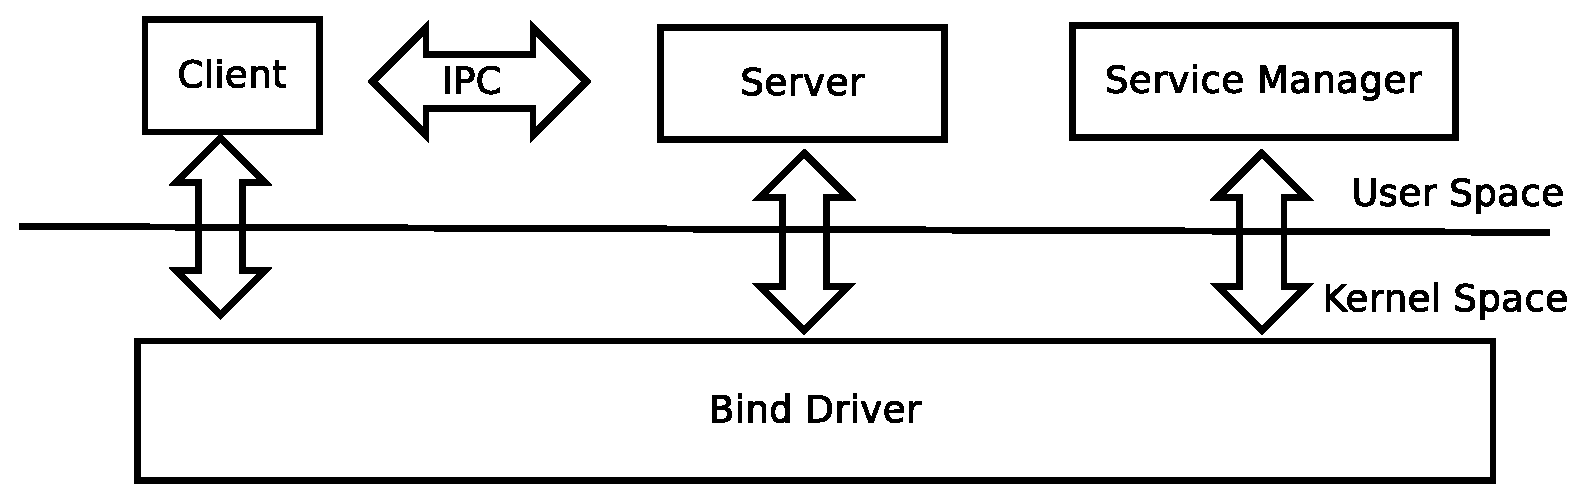
\includegraphics[keepaspectratio=true, scale=0.4]{dia/binder_model.eps}
    \caption{binder通信模型}
    \end{figure}

    Binder驱动基于RPC通信模型,即采用C/S模式,其模型类似于我们常用的网络通信。Binder框架定义了四个角色:Server,Client,Service Manager以及驱动。
    其中 Server,Client,Service Manager运行于用户空间,驱动运行于内核空间。这四个角色的关系和互联网类似:Server是服务器,Client是客户终端,Service Manager是域名服务器(DNS),驱动是路由器。

\section{C++库}
    \subsection{引用}
    \subsubsection{sp$<type>$ 以及wp$<type>$}
    %\subsection{sp$<type>$ 以及wp\textless type\textgreater}
    Android中定义了两种智能指针类型,一种是强指针sp(strong pointer),一种是弱指针(weak pointer)。其实称为强引用和弱引用更合适一些。强指针与一般意义的智能指针概念相同,通过引用计数来记录有多少使用者在使用一个对象,如果所有使用者都放弃了对该对象的引用,则该对象将被自动销毁。

    弱指针也指向一个对象,但是弱指针仅仅记录该对象的地址,不能通过弱指针来访问该对象,也就是说不能通过弱指针来调用对象的成员函数或访问对象的成员变量。要想访问弱指针所指向的对象,需首先将弱指针升级为强指针(通过wp类所提供的promote()方法)。弱指针所指向的对象是有可能在其它地方被销毁的,如果对象已经被销毁,wp的promote()方法将返回空指针,这样就能避免出现地址访问错的情况。

    sp和wp实际上就是android为其c++实现的垃圾自动回收机制:%
    当为sp时表示该对象存在于内存之中一直到该对象所有的引用消失时才回收其对象;%
    当为wp时表示该对象曾经存在过,而当其强引用结束后即会被回收而不管弱引用是否存在,%
    用于那些对系统并不是十分critical的对象,内存不够时即可被回收。

    sp$<type>$的构造函数和析构函数:\\
    \begin{lstlisting}[language=C++]
    template<typename T>
    sp<T>::sp(T* other)
    : m_ptr(other)    
    {                
        if (other) other->incStrong(this);
    } 
    template<typename T>
    sp<T>::~sp()
    {
        if (m_ptr) m_ptr->decStrong(this);
    }
    \end{lstlisting}

    在构造函数中调用了incStrong(),在析构函数中调用的decStrong(),显然是管理引用计数的函数,但是sp类的中并没有定义这两个函数,这两个函数是在RefBase类中定义的,由此可以得出结论:
    {\color{red}要想使用sp$<T>$或者wp$<T>$, T必需要继承RefBase类才行}。

    相关头文件:\\
    include/utils/StrongPointer.h \\
    include/utils/RefBase.h

    \subsection{Binder 框架}
    考察一次Binder通信的全过程会发现,Binder存在于系统以下几个部分中:

    · 应用程序进程:分别位于Server进程和Client进程中

    · Binder驱动:分别管理为Server端的Binder实体和Client端的引用

    · 传输数据:由于Binder可以跨进程传递,需要在传输数据中予以表述

    \subsection{以MediaService的诞生为例来讲Binder}
    \subsubsection{三个组成部分}
    \begin{description}
        \item[-] ServiceManager \\ 这是Android OS的整个服务的管理程序
        \item[-] MediaService \\ 这个程序里边注册了提供媒体播放的服务程序MediaPlayerService,我们最后只分析这个
        \item[-] MediaPlayerClient \\ 这个是与MediaPlayerService交互的客户端程序
    \end{description}
    \subsubsection{MediaPlayerService}
    源码文件在:MediaService的源码文件在:framework/base/Media/\\MediaServer/Main\_mediaserver.cpp 

    源代码:\\
    \begin{lstlisting}[language=C++]
    int main(int argc, char** argv)
    {
        sp<ProcessState> proc(ProcessState::self());
        sp<IServiceManager> sm = defaultServiceManager();
        ALOGI("ServiceManager: %p", sm.get());
        AudioFlinger::instantiate();
        MediaPlayerService::instantiate();
        CameraService::instantiate();                                                                                                                                                             
        AudioPolicyService::instantiate();
        ProcessState::self()->startThreadPool();
        IPCThreadState::self()->joinThreadPool();
    }
    \end{lstlisting}




\section{驱动}
    \begin{figure}[h!]
    \centering
    \includegraphics[keepaspectratio=true, scale=0.4]{dot/driver_data_structure.ps}
    \caption{binder通信模型}
    \end{figure}


\section{使用}
    \subsection{cmd:service}


\section{未讨论的部分}
    \begin{enumerate}
        \item 安全
        \item 引用计数
    \end{enumerate}

\section{附}
    \subsection{参考文章}
    \begin{description}
        \item Android深入浅出之Binder机制 \\http://blog.csdn.net/innost/article/details/6124685
        \item 引用计数
    \end{description}
    \subsection{红黑树}
%\end{CJK} %有始有終
\end{CJK*} %有始有終
\end{document}

